\myChapter{Tree depth influence in RTS games}\label{chap:rts}
\minitoc\mtcskip
\vfill
\lettrine{R}{eal} Time Strategy (RTS) games are a type of videogame
where the play takes action in real time (that is, there are not
turns, as in chess). Well-known games of this genre are Age of
Empires\texttrademark~ or Warcraft\texttrademark. In this kind of game
the players have units, structures and resources and they have to
confront with other players to win battles. Artificial Intelligence
(AI) in these games is usually very complex, because they are dealing
with a lot of actions and strategies at the same time. % y esto es
                                % importante para la tesis
                                % porque... todo capítulo debe tener
                                % una introducción que lo relacione
                                % con la metodología y los algoritmos
                                % que constituyen LA TESIS. Hasta
                                % ahora, parece "Blancanieves y los
                                % siete enanitos" o bien "Osgiliath y
                                % todo lo que se me ha ocurrido hacer
                                % con él" - JJ

The {\em Planet Wars} game, presented under the Google AI Challenge 2010\footnote{\url{http://planetwars.aichallenge.org/}} has been used by several authors for the study of computational intelligence in RTS games
\cite{Lara2013mapgenerator,Mora2012Genebot,FernandezAres2012adaptive}. This
is because it is a simplification of the elements that are present in
the complex games previously mentioned (only one type of resource and
one type of unit). % Todo problema debe ser acompañado por una
                   % caracterización del mismo y una metodología par
                   % aaplicar LA TESIS a ese tipo de problema. la
                   % conclusión debe generalizar lo hallado en el
                   % capítulo. Y no sé si seguírmelo leyendo, porque
                   % si no haces esto una opción es simplemente
                   % eliminar el capítulo si no contribuye a LA
                   % TESIS. - JJ


 Although this game has been described in previous works
 \cite{Lara2013mapgenerator,Mora2012Genebot,FernandezAres2012adaptive},
 % pero no en esta tesis, así que resúmelo (si al final vas a meter
 % esto) - JJ
we summarize saying that the objective of the player is to conquer
enemy and neutral planets in a space-like simulator. Each player has
planets (resources) that produce ships (units) depending of a
growth-rate. The player must send these ships to other planets
(literally, crashing towards the planet) to conquer them. A player win
if he is the owner of all the planets. As requirements, only one
second is the limit to calculate next actions (this time windows is
called {\em turn}\footnote{Although in this work we are using this
  term, note that the game is always performed in real time.}), and no
memory about the previous turns must be used.  Figure \ref{fig:naves}
shows a screen capture of the game. % Hay que caracterizar el
                                % problema, situarlo en contexto. ¿Es
                                % fácil o difícil? ¿A qué otro
                                % problema se parece? ¿Cuál es el
                                % estado del arte? No puedes
                                % copy/pastear simplemente lo que
                                % hayas escrito en el paper - JJ

\begin{SCfigure}
%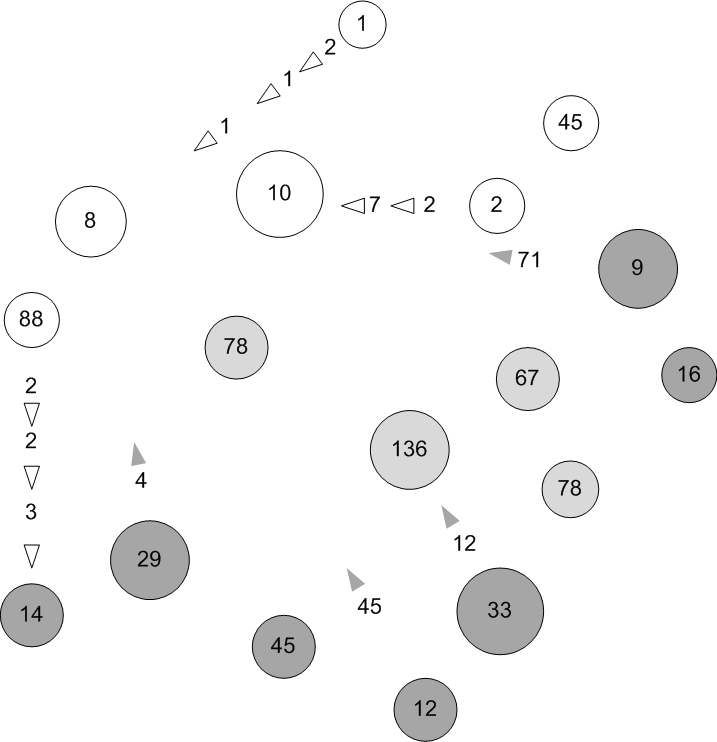
\includegraphics[scale=0.8]{gfx/rts/naves.bmp}

\caption{Example of execution of the Player Wars game. White planets and ships are owned by the player and dark gray ones are controlled by the enemy. Clear gray are neutral planets (not invaded).}
\label{fig:naves}
\end{SCfigure}


In this chapter we use Genetic Programming (GP) to obtain agents that play
Planet Wars game. % hala, así, sin vaselina ni nada. ¿Por qué GP? ¿Por
                  % qué no ES? ¿O cualquier otra cosa? 
The objective of GP is to create functions or programs to solve determined problems. Individual representation is usually in form of a tree, formed by operators (or {\em primitives}) and variables ({\em terminals}). These sets are usually fixed and known. The genome size is, therefore, variable, but the maximum size (depth) of the individuals is usually fixed, to avoid high evaluation costs. GP has been used to evolve LISP (LISt Processing) programs \cite{Koza1990Tools}, or XSLT (eXtensible Stylesheet Language Transformations) scripts \cite{Garcia2008XSLT}, among others.


We try to solve the next questions: 
\begin{itemize}
\item Can a tree-generated behaviour of an agent defeat an agent hand-coded by a player with experience and whose parameters have been also optimized?
\item Can this agent beats a more complicated opponent that is adapted to the environment?
\item How does the maximum depth affects the results?
\end{itemize}

The rest of the work is structured as follows: after the state of the art, the description of our agent is presented in Section \ref{sec:agent}. Then, the experimental setup conduced with the EA are showed (Section \ref{sec:experiments}). Finally, results, conclusions and future works are discussed.


%%%%%%%%%%%%%%%%%%%%%%%%SEC SOA
\section{Background}

RTS games have been used extensively in the computational intelligence area (see \cite{Lara2013review} for a review).
Among other techniques, Evolutionary Algorithms (EAs) have been widely used in computational intelligence in RTS games \cite{Lara2013review}. For example, for parameter optimization \cite{Esparcia10FPS}, learning \cite{Kenneth2005neuroevolution} or content generation \cite{Mahlmann2012MapGeneration}. 

One of these types, genetic programming, has been proved as a good tool for developing strategies in games, achieving results comparable to human, or human-based competitors \cite{Sipper2007gameplaying}. They also have obtained higher ranking than solvers produced by other techniques or even beating high-ranking humans \cite{Elyasaf2012FreeCell}. GP has also been used in different kind of games, such as board-games \cite{Benbassat2012Reversi}, or (in principle) simpler games such as Ms. Pac-Man \cite{Brandstetter2012PacMan} and Spoof \cite{Wittkamp2007spoof} and even in modern video-games such as First Person Shothers (FPS) (for example, Unreal\texttrademark~ \cite{Esparcia2013GPunreal}).


Planet Wars, the game we are going to use in this work, has been used as experimental environment for testing agents in other works. For example, in
\cite{Mora2012Genebot} the authors programmed the behaviour of a {\em bot} (a computer-controlled player) with a decision tree of 3 levels. Then, the values of these rules were optimized using a genetic algorithm to tune the strategy rates and percentages.  % ein????? - JJ - FERGU: re-escrito.
  Results showed a good performance confronting with other bots
  provided by the Google AI Challenge. 
  In \cite{FernandezAres2012adaptive} the authors improved this agent optimizing
  in different types of maps and selecting the set of optimized
  parameters depending of the map where the game was taking place,
  using a tree of 5 levels. These results outperformed the previous
  version of the bot with 87\% of victories. 

In this paper we use GP to create the decision tree,
instead of using our own gaming experience to model it, and compare
this agent with the two presented before.  



\section{Proposed Agent}
\label{sec:agent}


The proposed agent receives a tree to be executed. The generated tree
is a binary tree of expressions formed by two different types of nodes:

\begin{itemize}
\item {\em Decision}: a logical expression formed by a variable, a less than operator ($<$), and a number between 0 and 1. They are the equivalent to the ``primitives'' in the field of GP.
\item {\em Action}: the leaves of the the tree (therefore, the ``terminals''). Each decision is the name of the method to call that indicates to which planet send a percentage of available ships (from 0 to 1) from the planet that executes the tree. 
\end{itemize}

The different variables for the decisions are:

\begin{itemize}
\item {\em myShipsEnemyRatio}: Ratio between the player's ships and enemy's ships.
\item {\em myShipsLandedFlyingRatio}: Ratio between the player's landed and flying ships.
\item {\em myPlanetsEnemyRatio}: Ratio between the number of player's planets and the enemy's ones.
\item {\em myPlanetsTotalRatio}: Ration between the number of player's planet and total planets (neutrals and enemy included)-
\item {\em actualMyShipsRatio}: Ratio between the number of ships in the specific planet that evaluates the tree and player's total ships.
\item {\em actualLandedFlyingRatio}: Ratio between the number of ships landed and flying from the specific planet that evaluates the tree and player's total ships.
\end{itemize}

The decision list is:

\begin{itemize}
\item {\em Attack Nearest (Neutral|Enemy|NotMy) Planet}: The objective is the nearest planet.
\item {\em Attack Weakest (Neutral|Enemy|NotMy) Planet}: The objective is the planet with less ships.
\item {\em Attack Wealthiest (Neutral|Enemy|NotMy) Planet}: The objective is the planet with higher lower rate.
\item {\em Attack Beneficial (Neutral|Enemy|NotMy) Planet}: The objective is the planet more beneficial, that is the one with growth rate divided by the number of ships.
\item {\em Attack Quickest (Neutral|Enemy|NotMy) Planet}: The objective is the planet with higher facility to conquest: the lowest product between the distance from the planet that executes the tree and the number of the ships in the objective planet.
\item {\em Attack (Neutral|Enemy|NotMy) Base}: The objective is the planet with more ships (that is, the base).
\item {\em  Attack Random Planet}.
\item {\em Reinforce Nearest Planet}: Reinforce the nearest player's planet to the planet that executes the tree.
\item {\em Reinforce Base}: Reinforce the player's planet with higher number of ships.
\item {\em Reinforce Wealthiest Planet}: Reinforce the player's planet with higher grown rate.
\item {\em Do nothing}.


\end{itemize}

An example of a possible tree is shown in Figure \ref{fig:java}. This example tree has a total of 5 nodes, with 2 decisions and 3 actions, and a depth of 3 levels.

\begin{figure}[tb] 
\begin{center}
\begin{lstlisting}
if(myShipsLandedFlyingRatio<0.796)
	if(actualMyShipsRatio<0.201)
		attackWeakestNeutralPlanet(0.481);
	else
		attackNearestEnemyPlanet(0.913);
else
	attackNearestEnemyPlanet(0.819);
\end{lstlisting}
\end{center}
\caption{Example of a generated Java tree.}
\label{fig:java}
\end{figure}

The bot behaviour is explained in Figure \ref{alg:turn}.

\newsavebox{\algoartsbox}
\begin{lrbox}{\algoartsbox}
\begin{minipage}{10cm}
\begin{algorithmic}
%\COMMENT{At the beginning of the execution the agent receives the tree}
\STATE tree $\gets$ readTree()
\WHILE{$game not finished$}
  \STATE{starts the turn} %COMENTARIO!!!!
  \STATE {calculateGlobalPlanets()}%\tcp{e.g. Base or Enemy Base}\ %ARREGLAR
  \STATE {calculateGlobalRatios()}%\tcp{e.g. myPlanetsEnemyRatio}\
  \FOR{p in PlayerPlanets} %%%FOR EACH!
    \STATE calculateLocalPlanets(p)%\tcp{e.g. NearestNeutralPlanet to p}\
    \STATE calculateLocalRatios(p)%\tcp{e.g actualMyShipsRatio}\
    \STATE executeTree(p,tree)%\tcp{Send a percentage of ships to destination}\
  \ENDFOR

\ENDWHILE
\end{algorithmic}
\end{minipage}
\end{lrbox}

\begin{SCfigure}[20][htb]
\usebox{\algoartsbox}
\caption{Pseudocode of the proposed agent. The tree is fixed during all the agent's execution}
\label{alg:turn}
\end{SCfigure}






%\COMMENT {In each turn}
%\LOOP
	
%	\STATE calculateGlobalPlanets()
%	\COMMENT{{\em for example Base, Enemy Base...}}
%	\STATE calculateGlobalRatios ()
%	\COMMENT {{\em for example myPlanetEnemyRatio, myShipsEnemyRatio...}}
%		\FOR{each Planet: p}
%			\STATE calculateLocalPlanets (p)
%			\COMMENT{{\em for example NearestNeutralPlanet to planet p}}
%			\STATE calculateLocalRatios (p)
%			\COMMENT{{\em for example actualMyShipsRatio}}
%			\STATE executeTree(p,tree)
%			\COMMENT{{\em Send a percentage of the ships to another planet}}
%		\ENDFOR
%\ENDLOOP




\section{Experimental Setup}
\label{sec:experiments}

Sub-tree crossover and 1-node mutation evolutionary operators have been used, following other researchers' proposals that have used these operators obtaining good results \cite{Esparcia2013GPunreal}. In our case, the mutation randomly changes the decision of a node or mutate the value with a step-size of 0.25 (an adequate value empirically tested). Each configuration is executed 30 times, with a population of 32 individuals and a 2-tournament selector for a pool of 16 parents.

To test each individual during the evolution a battle with a previously created bot is performed in 5 different (but representative) maps provided by Google. Hierarchical fitness is used, as proposed in \cite{Mora2012Genebot}. Thus, an individual is better than another if it wins in a higher number of maps. In case of equality of victories, then the individual with more turns to be defeated (i.e. it is stronger) is considered better. The maximum fitness is, therefore 5 victories and 0 turns. Also, as proposed by \cite{Mora2012Genebot}, and due to the noisy fitness effect, in every generation all individuals are re-evaluated.


Two publicly available bots have been chosen for our experiments\footnote{Both can be downloaded from \url{https://github.com/deantares/genebot}}. The first bot to confront is {\em GeneBot}, proposed in \cite{Mora2012Genebot}. This bot was trained using a GA to optimize the 8 parameters that conforms a set of hand-made rules, obtained from an expert human player experience. The second one is an advanced version of the previous, called {\em Exp-Genebot} (Expert Genebot) \cite{FernandezAres2012adaptive}. This bot outperformed Genebot widely. Exp-Genebot bot analyses the distribution of the planets of the map to chose a previously optimized set of parameters by a GA.  Both bots are the best individual obtained of all runs of their algorithm (not an average one).

After running our algorithm without tree limitation in depth, it has also been executed with the lower and average levels obtained for the best individuals: 3 and 7, respectively, to study if this number has any effect on the results.   Table \ref{tab:parameters} summarizes all the parameters used.

\begin{table}
\begin{center}
\begin{tabular}{|c|c|}
\hline
{\em Parameter Name} & {\em Value} \\\hline
Population size & 32 \\\hline
Crossover type & Sub-tree crossover \\ \hline
Crossover rate & 0.5\\ \hline
Mutation  & 1-node mutation\\ \hline
Mutation step-size & 0.25 \\ \hline
Selection & 2-tournament \\ \hline
Replacement & Steady-state\\ \hline
Stop criterion & 50 generations \\ \hline
Maximum Tree Depth & 3, 7 and unlimited \\ \hline
Runs per configuration & 30 \\ \hline
Evaluation & Playing versus Genebot \cite{Mora2012Genebot} and Exp-Genebot \cite{FernandezAres2012adaptive} \\ \hline
Maps used in each evaluation & map76.txt map69.txt map7.txt map11.txt map26.txt \\ \hline
\end{tabular}
\caption{Parameters used in the experiments.}
\label{tab:parameters}
\end{center}
\end{table}

After all the executions we have evaluated the obtained best individuals in all runs confronting to the bots in a larger set of maps (the 100 maps provided by Google) to study the behaviour of the algorithm and how good are the obtained bots in maps that have not been used for training.

%The used framework is OSGiLiath, a service-oriented evolutionary
%framework. The generated tree is compiled in real-time and injected
%in the agent's code using Javassist library. All the source code used
%in this work is available under a LGPL V3 License in
%\url{http://www.osgiliath.org}. 
%Anda que ya te vale, cuando lo mencionas y resulta que lo borras - JJ

\section{Results}

Tables \ref{tab:resultsGenebot} and \ref{tab:resultsExpgenebot} summarize all the obtained results of the execution of our EA. These tables also show the average age, depth and number of nodes of the best individuals obtained and also the average population at the end of the run. The average turns rows are calculated only taking into account the individuals with lower victories than 5, because this number is 0 if they have win the five battles.



\begin{table*}
\centering{
\begin{tabular}{|c|c|c|c|c|} \hline
    \multicolumn{2}{|c|}{}    &  {\em Depth 3}                & {\em Depth 7}                &    {\em Unlimited  Depth}    \\ \hline  
\multirow{2}{*}{Best Fitness}  & Victories     &   \textbf{4.933} $\pm$ 0.25       &  4.83 $\pm$ 0.53       &    4.9     $\pm$ 0.30  \\ \cline{2-5}  
              & Turns         &  244.5 $\pm$  54.44     &  466   $\pm$ 205.44    &    266.667 $\pm$ 40.42 \\ \hline  
\multirow{2}{*}{Population Ave. Fitness}  & Victories     &   \textbf{4.486}$\pm$ 0.52 & 4.43 $\pm$ 0.07   &    4.711   $\pm$ 0.45  \\ \cline{2-5}  
              & Turns         &  130.77$\pm$ 95.81      &  139.43 $\pm$ 196.60   &    190.346 $\pm$ 102.92\\ \hline  
\multirow{2}{*}{Depth}         & Best          &  3     $\pm$ 0          & 5.2 $\pm$ 1.78         &    6.933   $\pm$ 4.05  \\ \cline{2-5}
              & Population    &  3  $\pm$ 0             & 5.267 $\pm$ 1.8        &    7.353   $\pm$ 3.11  \\ \hline  
\multirow{2}{*}{Nodes}         & Best          &  7     $\pm$ 0          &   13.667 $\pm$ 7.68    &    22.133  $\pm$ 22.21 \\ \cline{2-5}  
              & Population    &  7     $\pm$ 0          & 13.818 $\pm$ 5.86      &    21.418  $\pm$ 13.81 \\ \hline  
\multirow{2}{*}{Age}           & Best          &  \textbf{8.133} $\pm$ 3.95       & 5.467 $\pm$ 2.95       &    5.066   $\pm$ 2.11  \\ \cline{2-5}
              & Population    &  \textbf{4.297} $\pm$ 3.027      & 3.247 $\pm$ 0.25       &    3.092   $\pm$ 1.27  \\ \hline
\end{tabular}
\caption{Average results obtained from each configuration versus Genebot. Each one has been tested 30 times.}
\label{tab:resultsGenebot}
}
\end{table*}

\begin{table*}
\centering{
\begin{tabular}{|c|c|c|c|c|} \hline            
 \multicolumn{2}{|c|}{}        &  {\em Depth 3}                & {\em Depth     7}            &   {\em Unlimited Depth}     \\ \hline  
\multirow{2}{*}{Best Fitness}  & Victories     &   4.133   $\pm$ 0.50    & 4.2      $\pm$ 0.48    &   \textbf{4.4}     $\pm$ 0.56  \\ \cline{2-5} 
              & Turns          &  221.625 $\pm$ 54.43   & 163.667  $\pm$ 106.38  &   123.533 $\pm$ 112.79\\ \hline 
\multirow{2}{*}{Population Ave. Fitness}  & Victories      &  3.541   $\pm$ 0.34    & 3.689    $\pm$ 0.37    &   \textbf{4.043}   $\pm$ 0.38  \\ \cline{2-5} 
              & Turns          &  200.086 $\pm$ 50.79   & 184.076  $\pm$ 57.02   &   159.094 $\pm$ 61.84 \\ \hline  
\multirow{2}{*}{Depth}         & Best           &  3       $\pm$ 0       & 5.2      $\pm$ 1.84    &   6.966   $\pm$ 4.44  \\ \cline{2-5} 
              & Population     &  3       $\pm$ 0       & 5.216    $\pm$ 0.92    &   6.522   $\pm$ 1.91  \\ \hline 
\multirow{2}{*}{Nodes}         & Best           &  7       $\pm$ 0       & 12.6     $\pm$ 6.44    &   18.466  $\pm$ 15.46 \\ \cline{2-5}   
              & Population     &  7       $\pm$ 0       & 13.05    $\pm$ 3.92    &   16.337  $\pm$ 7.67  \\ \hline 
\multirow{2}{*}{Age}           & Best           &  4.266   $\pm$ 5.01    & 4.133    $\pm$ 4.26    &   \textbf{4.7}     $\pm$ 4.72  \\ \cline{2-5} 
              & Population     &  3.706   $\pm$ 0.58    & 3.727    $\pm$ 0.62    &   \textbf{3.889}   $\pm$ 0.71  \\ \hline  


\end{tabular}
\caption{Average results obtained from each configuration versus Exp-Genebot. Each one has been tested 30 times.}
\label{tab:resultsExpgenebot}
}
\end{table*}

As can be seen, versus Genebot, the average population fitness is nearest to the optimum than versus Exp-Genebot, even with the lowest depth. Highest permanence in the population is also with the depth of 3 levels. On the contrary, confronting with Exp-Genebot the configuration with unlimited depth achieves better results. This make sense because more decisions should be taken because the enemy can be different in each map.

In the second experiment, we have confronted the 30 bots obtained in each configuration again with Genebot and Exp-Genebot, but in the 100 maps provided by Google. This has been used to validate if the obtained individuals of our method can be competitive in terms of quality in maps not used for evaluation. Results are shown in Table \ref{tab:allmaps} and boxplots in Figure \ref{fig:victories}. It can be seen that in average, the bots produced by our algorithm perform equal or better than the best obtained by the previous authors. Note that, even obtaining individuals with maximum fitness (5 victories) that have been kept in the population several generations (as presented 
before in Tables \ref{tab:resultsGenebot} and \ref{tab:resultsExpgenebot}) cannot be representative of a extremely good bot in a wider set of maps that have not been used for training. As the distributions are not normal, a Kruskal-Wallis test has been used, obtaining significant differences in turns for the experiment versus Genebot (p-value = 0.0028) and victories in Exp-genebot (p-value = 0.02681). Therefore, there are differences using a maximum depth in the generation of bots. In both configurations, the trees created with 7 levels of depth as maximum have obtained the better results.

To explain why results versus Genebot (a weaker bot than Exp-Genebot) are slightly worse than versus Exp-Genebot, even when the best individuals produced by the GP have higher fitness, we have to analyse how the best individual and the population are being evolved. Figure \ref{fig:gens} shows that best individual using Genebot reaches the optimal before Exp-Genebot, and also the average population converges quicker. This could lead to over-specialization: that is, the generated bots are over-trained to win in the five maps, and because re-evaluation these individuals are still changing after they have reached the optimal.



\begin{table*}
\centering{
\begin{tabular}{|c|c|c|c|c|c|c|} \hline
   
    
  


{\em Configuration}     &    {\em Average maps won}  &    {\em Average turns}     \\ \hline
                   \multicolumn{3}{|c|}{Versus Genebot}    \\ \hline
 Depth 3          &   47.033 $\pm$ 10.001 &   133.371 $\pm$   16.34    \\ \hline
 Depth 7          &   48.9 $\pm$ 10.21    &   \textbf{141.386} $\pm$  15.54   \\ \hline
 Unlimited Depth  &   50.23 $\pm$ 11.40   &   133.916   $\pm$   10.55    \\ \hline
       \multicolumn{3}{|c|}{Versus Exp-Genebot}                          \\ \hline              
 Depth 3          &   52.367 $\pm$ 13.39 &  191.051 $\pm$ 67.79 \\ \hline
 Depth 7          &   \textbf{58.867} $\pm$ 7.35  &  174.694$\pm$ 47.50 \\ \hline
 Unlimited Depth  &   52.3 $\pm$ 11.57   &  197.492 $\pm$ 72.30 \\ \hline 

\end{tabular}


\caption{Results confronting the 30 best bots attained from each configuration in the 100 maps each.}
\label{tab:allmaps}
}
\end{table*}

\begin{figure}[htb]
\centering

%\subfigure[Victories]{
   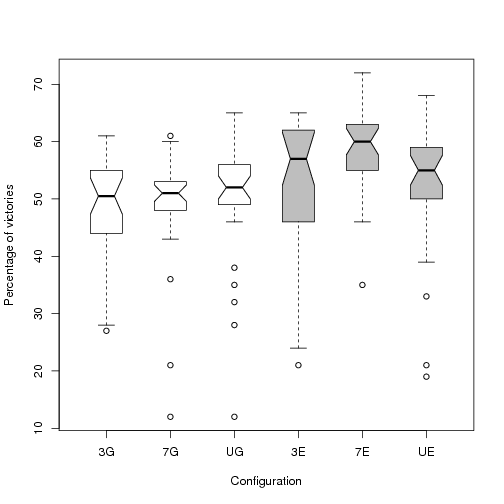
\includegraphics[scale =0.30] {gfx/rts/victories.png}
   \label{fig:subfig1}
 %}
%\subfigure[Turns]{
   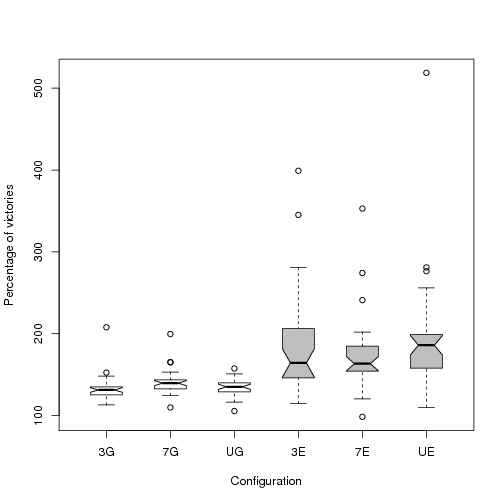
\includegraphics[scale =0.30] {gfx/rts/turns.png}
   \label{fig:subfig2}
 %}
\caption{Average of executing the 30 best bots in each configuration (3, 7 and U) versus Genebot (G) and Exp-Genebot (E).}

\label{fig:victories}
\end{figure}

\begin{figure}[htb]
\centering
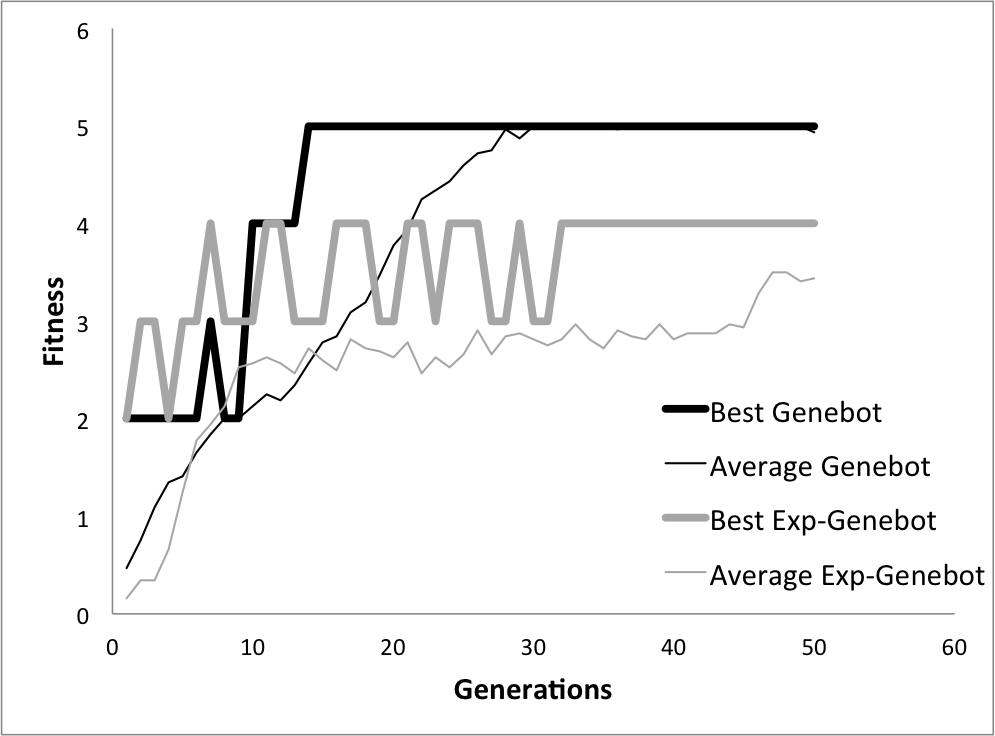
\includegraphics[scale =0.60] {gfx/rts/generations.png}
\caption{Evolution of the best individual and the average population during one run for depth 7 versus Genebot and Exp-Genebot.}
\label{fig:gens}
\end{figure}
 
\section{Conclusions}
\label{sec:conclusion}

This work presents a Genetic Programming algorithm that generates
agents for playing Planet Wars game. A number of possible actions to
perform and decision variables have been presented. We have used two
competitive bots available in the literature (Genebot and Exp-Genebot)
to calculate the fitness of the generated individuals. These two bots
were the best obtained from several runs and the behaviour to optimize
was extracted from human expertise. Three different maximum depth for
the trees have been used: 3, 7 and unlimited. Results show that best
individuals outperforms these agents during the evolution in all
configurations. These individuals have been tested against a larger
set of maps not previously used during the evolution, obtaining
equivalent or better results than Genebot and Exp-Genebot. 
% Las conclusiones del trabajo explícito no sirven. Debes de sacar
% conclusiones de la aplicación de una metodología a un problema
% específico y generalizar para problemas de esa clase. También tienes
% que mostrar como TU TESIS ha contribuido, de forma decisiva, a la
% solución de ese problema. - JJ

In future work, other rules will be added to our algorithm (for
example, the ones that analyse the map, as the Exp-Genebot does) and
different enemies will be used. Other games used in the area of
computational intelligence in videogames, such as
Unreal\texttrademark~ or Super Mario\texttrademark~ will be tested.
% Borra future work en la tesis.